\label{sec:background}

Figure \ref{fig:hipster} gives an overview of the Hipster system. Starting from an Isabelle theory file, defining a set of datatypes and functions, the user calls Hipster on list of functions about which she is interested in finding lemmas. The workings of Hipster can be divided up into three stages:
\begin{enumerate}
\item Generation of Haskell code. 
\item Theory exploration in Haskell.
\item Proof in Isabelle.
\end{enumerate}
Hipster uses Isabelle's code generator \cite{codegen}, to translate the theory to a Haskell program. Hipster is then using the theory exploration system HipSpec as a backend for generating conjctures. While HipSpec can be used also as a fully fledged theorem prover, Hipster only use its conjecture generation subsystem QuickSpec \cite{quickspec}, and performs proofs inside Isabelle. Isabelle is an LCF-style prover, which means that it is based on a small core of trusted axioms, upon which subsequent proofs must be built. Therefore, any proofs found outside Isabelle, e.g. by HipSpec would have to be reconstructed inside Isabelle anyway, hence it is easier for Hipster to simply use Isabelle for proofs in the first place. 
\begin{figure}[htbp]
\begin{center}
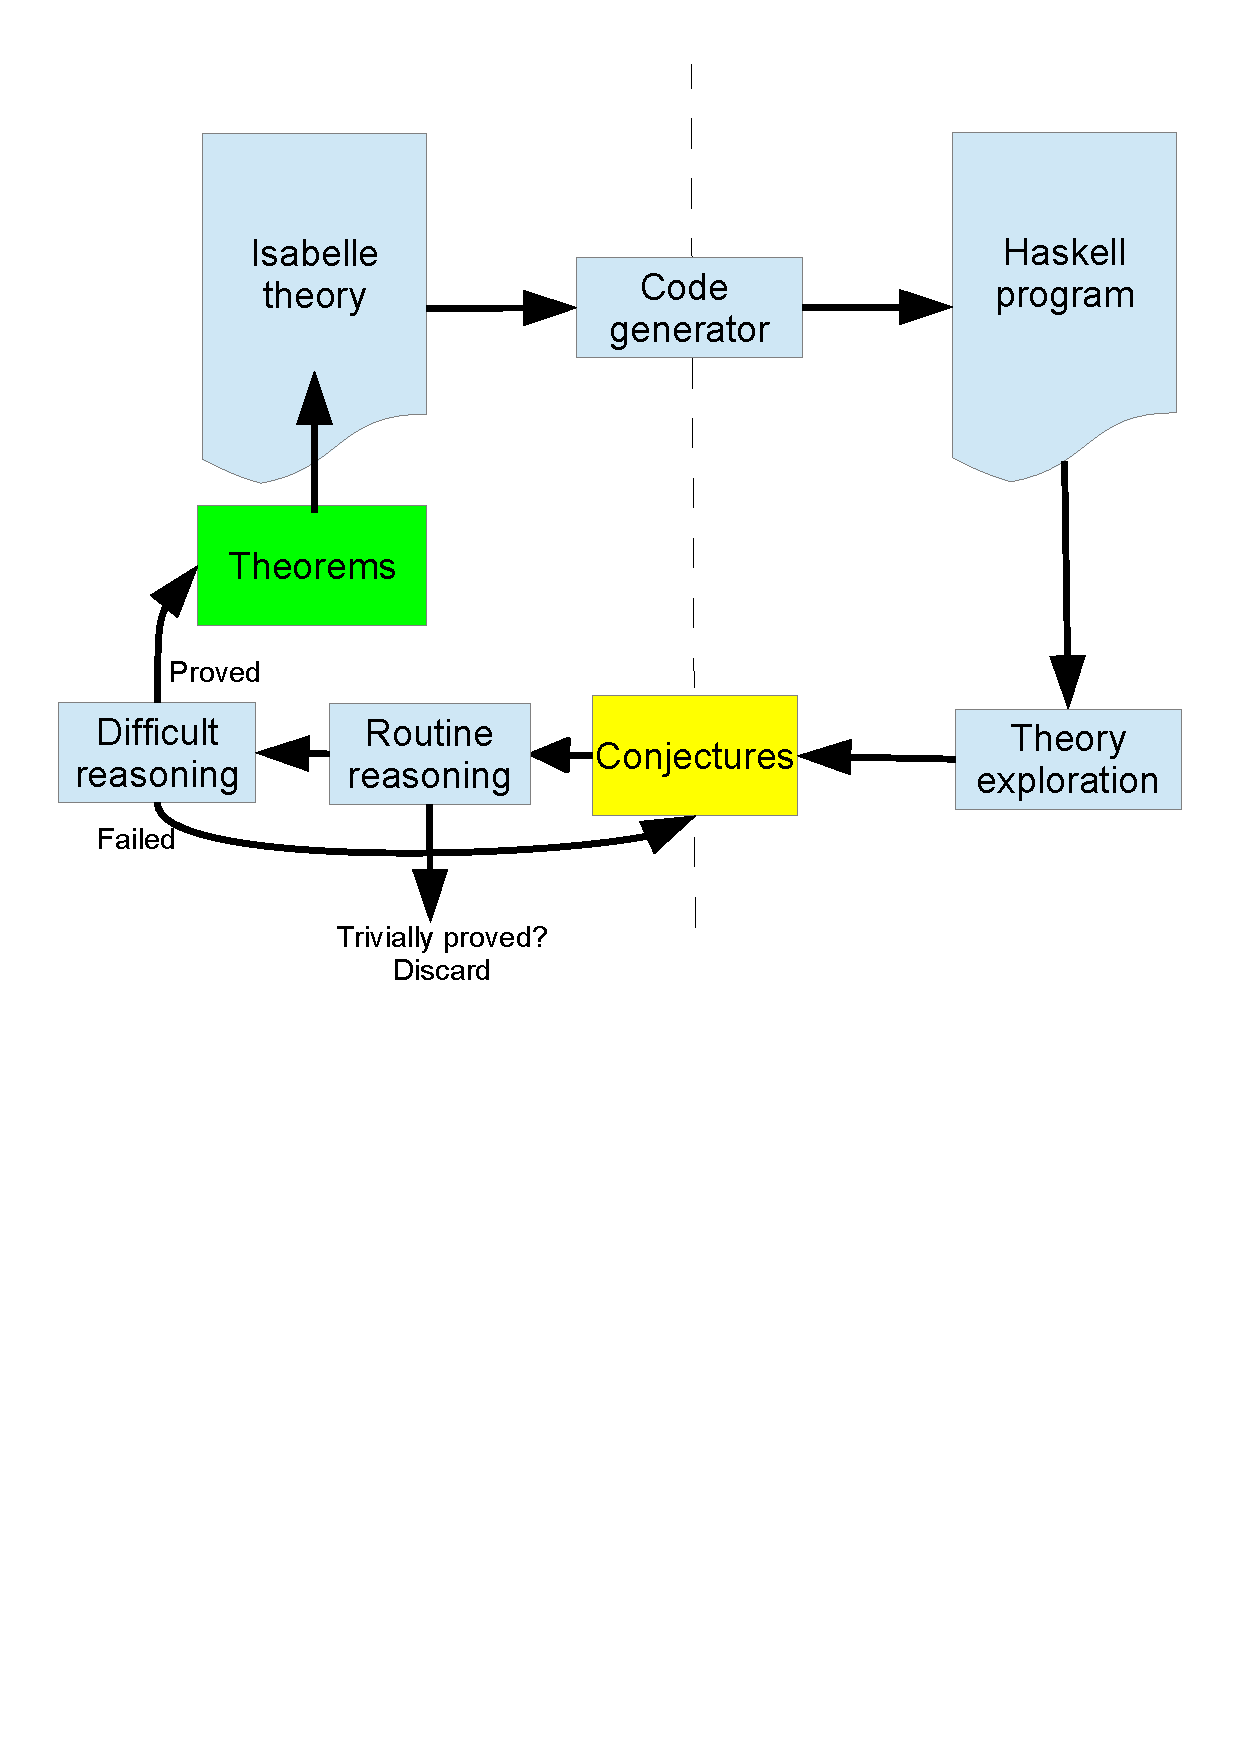
\includegraphics[scale=0.4]{hipster}
\caption{Overview of Hipster}
\label{fig:hipster}
\end{center}
\end{figure}

Not all conjectures returned from QuickSpec are interesting. Hipster is parametrised by two tactics, which can be set by the user: one for \emph{routine reasoning} and one for \emph{difficult reasoning}. Conjectures solved by routine reasoning are deemed trivial and discarded, while those requiring more difficult reasoning are displayed to the user and included in the Isabelle theory so they can be used in subsequent proofs if necessary. In the context of this paper, routine reasoning is first-order equational reasoning and simplification, while difficult reasoning involves some kind of induction. Occasionally, Hipster might discover some conjecture which it cannot prove automatically. Such an open conjecture would also be displayed to the user, who can then choose to perform an interactive proof.

